% vim:set shiftwidth=2 tabstop=2 expandtab:

\chapter{Nonlinear cointegrating regressions with nonstationary time series}
\ifpdf
    \graphicspath{{Chapter6/Chapter6Figs/PNG/}{Chapter6/Chapter6Figs/PDF/}{Chapter6/Chapter6Figs/}}
\else
    \graphicspath{{Chapter6/Chapter6Figs/EPS/}{Chapter6/Chapter6Figs/}}
\fi

\section{Introduction}
The past few decades has witnessed significant developments in cointegration analysis.
 In particular, extensive researches  have been focused on cointegration models with linear structure. Whilst it is convenient for practical implementation, nonetheless, it is restrictive, especially in the context of economics, often suggesting nonlinear responses with some unknown parameters.
For empirical examples, we refer to   \cite{grangerterasvirta1993} as well as \cite{terasvirtatjostheimgranger2010}. In this situation, it is expected that nonlinear cointegration captures the features of many long-run relationships
in a more realistic manner.

A typical non-linear parametric cointegrating regression model has the form
\be
  y_t&=& f(x_t, \theta_0)+\,  u_t, \quad t=1,...,n\la{eqn:6:intro}.
\ee
where  $f:\mathbb{R} \times \mathbb{R}^m \rightarrow \mathbb{R}$ is a known nonlinear function, $x_t$ and  $u_t$ are regressor and regression errors, and   $\theta_0$ is an $m$-dimensional true parameter vector that lies in the parameter set $\Theta$. With the observed data $\{y_t, x_t\}_{t=1}^n$, which may include non-stationary components, this paper is concerned with the nonlinear least square (NLS) estimation of the unknown parameters $\theta\in \Theta$. In this regard, \cite[][\citeyear{parkphillips2001}]{parkphillips1999}, PP henceforth, considers $x_t$ to be an integrated $I(1)$ process. Based on PP framework, \cite{changparkphillips2001} introduced additional linear time trend term and stationary regressors into model (\ref{eqn:6:intro}). \cite{changpark2003} extends to nonlinear index models driven by integrated process.  More recently, \cite{choisaikkonen2010}, \cite{gaokinglutjostheim2009} and \cite{wangphillips2012} developed statistical tests  for the existence of nonlinear cointegrating relation. \cite{changpark2010} allows the regressors $x_t$ to be contemporaneous correlated with the regression errors $u_t$. \cite{shiphillips2010} extends the model (\ref{eqn:6:intro}) and incorporates a loading coefficient.


The present paper has a similar goal to the previous mentioned papers but offers more general results that we hope has some advantage. First of all, we establish a general framework for  weak consistency of the NLS estimator $\hat{\theta}_n$, allowing for the $x_t$ to be  a  wider class of non-stationary time series.
 The set of sufficient conditions are easy to apply to various non-stationary regressors, including partial sum of linear process and recurrent Markov chain. Furthermore, we  provide a limit distribution for the NLS estimator $\hat{\theta}_n$. It  deserves to mention that  the routine in this paper to establish the limit distribution of $\hat\theta_n$ is different from previous work, e.g. \cite{parkphillips2001}. Roughly speaking, our routine is related to joint distributional convergence of a martingale under target and its conditional variances, rather than using classical martingale limit theorem by establishing the convergence in probability for the conditional variance.  In nonlinear co-integrating regression, there are   some advantages for our methodology  since it is usually difficult to establish the convergence in probability for the conditional variance, in particular, in the situation that the regressor $x_t$ is a non-stationary time series.

Second, in addition to the commonly used martingale innovation structure, our model allows for serial dependence in the equilibrium errors $u_t$ and the innovations driving $x_t$. It is important as our model  permits joint determination of $x_t$ and $y_t$, and hence the system is a time series structural model. Under such situation, the weak consistency and limit distribution of the NLS estimator $\hat{\theta}_n$ are also established.

This paper is organized as follow. Section 2 presents our main results of weak consistency. The results on limit distribution of the NLS estimator are given in Section 3. Extension to endogeneity is presented in Section 4. Technical proofs are postponed to Section 6. Throughout the paper, we denote constants by $C, C_1, C_2,...$ which may be different at each appearance, and assume that $\|x\|=(x_1^2+...+x_m^2)^{1/2}$ whenever $x=(x_1,...,x_m)$. Furthermore,  the parameter set $\Theta \subset \mathbb {R}^m$ is assumed to be compact and convex, and the true parameter vector $\theta_0$ is an interior point of $\Theta$.



\section {Weak consistency}
This section considers the estimation of the unknown parameters $\theta$ in model (\ref {eqn:6:intro}) by NLS.
Let $Q_n(\theta) = \sum_{t = 1}^n ( y_t - f(x_t, \theta))^2$. The NLS estimator $\hat\theta_n$ of $\theta$
is defined to be the minimizer of $Q_n(\theta)$ over $\theta \in \Theta$, that is,
\be
\hat{\theta}_n = \arg{\min}_{\theta \in \Theta} Q_n(\theta) , \la{eqn:6:sad2}
\ee
and the error estimate is defined by $\hat{\si}_n^2 = n^{-1} \sum_{t = 1}^n \hat{u}_t^2$, where $\hat{u}_t = y_t - f(x_t, \hat{\theta}_n)$. To investigate the weak consistency for the NLS estimator $\hat\theta_n$,
this section assumes the  regression model (\ref {eqn:6:intro}) having a martingale structure.
In this situation, our sufficient conditions are  closely related  to those of \cite{wu1981}, \cite{lai1994} and \cite{skouras2000}, which provides a general framework. In comparison to the papers mentioned,   our assumptions are  easy to apply, particularly in non-linear cointegrating regression situation, as stated in two examples below. Extension to endogeneity between $x_t$ and $u_t$ is investigated in Section 4.

\subsection{Main results}
We make use of the following assumptions for the development of the weak consistency.



\begin{assump} \la{assump:6:Convex}
For each $\pi,\pi_0 \in \Theta$, there exists a real function $T:\mathbb{R} \rightarrow \mathbb{R}$ such that
\be
|f(x, \pi) - f(x, \pi_0)| \le h(||\pi - \pi_0||) T(x), \la{eqn:6:45}
 \ee
 where $h(x)$ is a bounded real function such that $h(x)\downarrow h(0)=0$, as $x\downarrow 0.$
\end{assump}

\begin{assump} \la{assump:6:Martingale}
(i) $\{u_{t},\mathcal{F}_{t},1\leq t\leq n\}$ is a martingale
difference sequence satisfying
$E(|u_t|^2|\mathcal{F}_{t-1}) = \si^2$, $\sup_{1\leq t\leq n}E(|u_{t}|^{2q}|\mathcal{F}_{t-1})<\infty$ a.s., where $q > 1$; (ii) $x_t$ is adapted to $\F_{t - 1}$, $t = 1, ..., n$.
\end{assump}

\begin{assump} \la{eqn:6:assumpLowerBound} There exists an increasing sequence $0<\kappa_n \to \infty$ such that
 \be\kappa_n^{-2} \sum_{t = 1}^n [T(x_t) + T^2(x_t)] = O_P(1), \la{20}\ee and for any $0<\eta<1$ and $\theta \ne \theta_0$, where $\theta, \theta_0\in \Theta$, there exist
 $n_0 > 0$ and $M_1>0$ such that
\be
P \Big ( \sum_{t = 1}^n ( f(x_t, \theta) - f(x_t, \theta_0))^2 \ge \kappa_n^2\,/ M_1 \Big ) \ge 1 - \eta, \la{eqn:6:21}
\ee
 for   all $n > n_0$.
\end{assump}

\begin{thm} \la{thmConsistency} Under Assumption \ref{assump:6:Convex}--\ref{assump:6:LowerBound}, the NLS estimator $\hat{\theta}_n$ is a consistent estimator of $\theta_0$, i.e. $\hat{\theta}_n \rightarrow_P \theta_0$.

If in addition $\kappa_n^2 n^{-1} = O_P(1)$, then $\hat{\si}^2_n \to_P \si^2$, as $n \to \infty$.
\end{thm}

Assumptions \ref {assump:6:Convex} and \ref{assump:6:Martingale} are the same as in
 \cite{skouras2000}, which are standard in the NLS estimation theory. Also see \cite{wu1981} and \cite{lai1994}. Assumption \ref {assump:6:LowerBound} is used to replace (3.8), (3.9) and (3.11) in \cite{skouras2000} in which some uniform conditions are used. In comparison to \cite{skouras2000}, Assumption \ref {assump:6:LowerBound}, which is related to the conditions on the regressor $x_t$, is more natural and easy to apply, particularly in the situation that $T(x)$ is integrable and the regressor $x_t$ is an non-stationary time series, as stated in the following examples.

\medskip
{\bf Example 1 (Partial sum of linear process).}
Let $x_{t}=\sum_{j=1}^t \xi_{j}$, where $\{\xi _{j},j\geq 1\}$ is a linear process
defined by
\begin{equation}
\xi _{j}=\sum_{k=0}^{\infty }\,\phi _{k}\,\epsilon _{j-k}, \la{eqn:6:sec2.f1}
\end{equation}
where $\{\epsilon _{j},-\infty <j<\infty \}$ is a sequence of iid
random variables with $E\epsilon _{0}=0$, $E\epsilon _{0}^{2}=1$ and the
characteristic function $\varphi (t)$ of $\epsilon _{0}$ satisfies
$\int_{-\infty
}^{\infty }|\varphi (t)|dt<\infty $.
The coefficients $\phi_k$ are assumed to satisfy one of the following conditions:

{\textbf{C1.}} $\phi_k \sim  k^{-\mu} \rho(k)$, where $1 / 2 < \mu < 1$ and $\rho(k)$ is a function slowly varying at $\infty$.

{\textbf{C2.}} $\sum_{k=0}^{\infty }|\phi _{k}|<\infty $ and $\phi \equiv \sum_{k=0}^{\infty }\phi_{k}\not =0$.

\noindent Put $d_n^2 = \E x_n^2.$ As in \cite{wanglingulati2003}, we have
\be
d_n^2 = \E x_n^2 \sim
\begin{cases}
c_{\mu} n^{3-2\mu} \rho^2(n),  & \mbox{under C1,} \\
\phi^2 n, & \mbox{under C2.}
\end{cases}
\ee
where $c_\mu = 1 / ((1 - \mu)(3-2\mu )) \int_{0}^{\infty} x^{-\mu} (x+1)^{-\mu} dx$.

We have the following result.

\begin{thm} \la{thmLinearConsistency} If $T(x)$ is bounded and integrable and
$
\int_{-\infty}^{\infty} (f(s, \theta) - f(s, \theta_0))^2 ds>0
$
for all $\theta\not=\theta_0$, then (\ref {eqn:6:20}) and (\ref {eqn:6:21}) hold with $\kappa^2_n=n/d_n$.
\end{thm}


  Theorem 2.2  improves Theorem 4.1 of PP in two folds.
First we allow for more general regressor. The result under {\bf C1} is new, which allows $x_t$ to be long memory process, including the fractionally integrated process as an example. PP only allows $x_t$ to satisfy {\bf C2} with additional conditions on $\phi_k$, that is, requires $x_t$ to be a partial sum of short memory process. Secondly we remove the part (b) required in the definition of I-regular function given in their Definition 3.3. PP requires $f(x, \theta)$ to be piecewise smooth and we only require the $[f(s, \theta)-f(s, \theta_0)]^2$ to be integrable.



\medskip
{\bf Example 2  (Recurrent Markov Chain).}
Let $\{x_k\}_{k\ge 0}$ be a Harris recurrent Markov chain with state space $(E, \mathcal{E})$,
transition probability $P(x, A)$ and invariant measure $\pi$. We denote $P_\mu$ for the Markovian probability
with the initial distribution $\mu$, $E_\mu$ for correspondent expectation and $P^k(x, A)$
for the $k$-step transition of $\{x_k\}_{k\ge 0}$.  A subset $D$ of $E$ with $0<\pi(D)<\infty$ is called $D$-set of $\{x_k\}_{k\ge 0}$ if for any $A\in \mathcal{E}^+$,
$$
\sup_{x\in E} E_x\big(\sum_{k=1}^{\tau_A}I_D(X_k)\big)<\infty,
$$
where $ \mathcal{E}^+=\{A\in  \mathcal{E}: \pi(A)>0\}$ and $\tau_A=\inf\{n\ge 1: \ x_n\in A\}$. As is well-known,
$D$-sets not only exist,  but generate the entire sigma $\mathcal{E}$, and
 for any $D$-sets $C, D$ and any probability measure $\nu, \mu$ on $(E, \mathcal{E})$,
\be
\lim_{n\to\infty}\sum_{k=1}^n\nu P^k(C)/\sum_{k=1}^n\mu P^k(D) &=&\frac {\pi (C)}{\pi (D)}, \la{eqn:6:1.3}
\ee
where $\nu P^k(D) =\int_{-\infty}^{\infty} P^k(x, D)\nu(dx)$. See \cite{nummelin2004} for instance.

Let a $D$-set $D$ and a probability measure $\nu$ on $(E, \mathcal{E})$ be fixed. Define
\bestar
a(t) &=& \pi^{-1}(D)\sum_{k=1}^{[t]}\nu P^k(D), \quad t\ge 0.
\eestar
 By recurrence, $a(t)\to\infty$. Here and below, we set the state space to be the real space, that is $(E, \mathcal{E}) = (R, \mathcal{R})$. We have the following result.

\begin{thm} \la {thmMarkovConsistency}If $T(x)$ is bounded and $\int_{-\infty}^{\infty} |T(x)|\pi(dx) < \infty$ and
$
\int_{-\infty}^{\infty} (f(s, \theta) - f(s, \theta_0))^2 \pi(ds)>0
$
for all $\theta\not=\theta_0$, then (\ref {eqn:6:20}) and (\ref {eqn:6:21}) hold with $\kappa^2_n=a(n)$.

\end{thm}

Theorem \ref {thmMarkovConsistency} seems to be new to literature. By virtue of (\ref {eqn:6:1.3}), the asymptotic order of $a(t)$ depends only on $\{x_k\}_{k\ge 0}$.
It is interesting to notice that Theorem \ref {thmMarkovConsistency} does not impose the $\beta$-regular condition as common used in literature. The Harris recurrent Markov chain $\{x_k\}_{k\ge 0}$  is called $\beta$-regular if
\be
\lim_{\lam\to \infty} a(\lam t)/a(\lam) &=&t^\beta,\quad \forall t>0, \la{eqn:6:d1}
\ee
where $0< \beta\le 1$. See \cite{chen1999} for instance.


\begin{rem} Although we assume the integrability,
Theorem 2.1 allows for certain non-integrable $f(x, \theta)$. For instance, if $f(x, \theta)=\theta \, x^{\al}$, where $\al>0$ is given, (\ref {eqn:6:45}) holds with $h(x)=|x|$ and $T(x)=|x^{\al}|$.
 Under  $x_t/d_n \Rightarrow_D G(t)$ on $D[0,1]$, where $G(t)$ is  some continuous stochastic process,  it follows from the continuous mapping theorem that
\be
  \frac{1}{n} \sum_{t = 1}^n (x_t/d_n)^{2\al}  \to_D \int_{0}^{1} G(t)^{2\al} dt
\ee
on $D[0,1]$, which implies the required (\ref{eqn:6:20}) and (\ref{eqn:6:21}) with $\kappa^2_n = n\,d_n^{\,2\al}$.
\end{rem}

However, some modifications to our Theorem 2.1 are necessary for establishing the weak consistency of the $\hat\theta_n$, under  more general non-integrable $f(x, \theta)$. In this regard, we follow PP to consider the asymptotic homogeneous function.

Let $f:\mathbb{R} \times \Theta \rightarrow \mathbb{R} $ have the structure:
 \be
 f(\lambda x, \theta) = v(\lambda, \theta) h(x,\theta) + b(\lambda, \theta)\, A(x, \theta)\, B(\lambda x, \theta), \la{eqn:6:sad1}
 \ee
 where $\sup_{\theta\in \Theta}|b(\lambda, \theta)\, v^{-1}(\lambda, \theta)|\to 0$, as $\lambda\to \infty$; $\sup_{\theta\in \Theta}|A(x, \theta)|$ is locally bounded, that is, bounded on bounded intervals;
 $\sup_{\theta\in \Theta} |B(\lambda x, \theta)|$ is bounded on $R$; $h(x, \theta)$ is regular on $\Theta$ (see Appendix for definition of regularity) and $v(\lambda, \theta)$ belongs to one of the following cases:

 {\bf Case 1} (i) $v(\lambda, \theta)  = v(\lambda)$ and $v(\lambda)$ is bounded away from zero as $\lambda \to \infty$; (ii) for all $\theta \ne \theta_0$ and $\de > 0$, $\int_{|s| \le \de} (h(s, \theta) - h(s, \theta_0))^2 ds > 0$.

 {\bf Case 2} (i) for any $\bar{\theta} \ne \theta_0$ and $\bar{p}, \bar{q} > 0$, there exist $\ep > 0$ and a neighborhood $N$ of $\bar{\theta}$ such that as $\lambda \to \infty$
\be
\inf_{\substack{|p-\bar{p}| < \ep \\ |q-\bar{q}| < \ep}} \inf_{\theta \in N} |p v(\lambda, \theta) - q v(\lambda, \theta_0) | \to \infty;
\ee
(ii) for all $\theta \ne \theta_0$ and $\de > 0$, $\int_{|s| \le \de} h^2(s, \theta)  ds > 0$.


\begin{thm} \la {thmHomoConsistent1} Suppose that $f(x, \theta)$ in model (\ref {eqn:6:intro}) has the structure (\ref {eqn:6:sad1}), and in addition to Assumption 2.2, there exists a continuous Gaussian process $G(t)$ such that $x_{[nt], n} \Rightarrow_D G(t)$, on $D[0,1]$, where $x_{i,n} = x_i / d_n$  and $0 < d_n \to \infty$ is a sequence of real numbers. Then,
 the NLS estimator $\hat{\theta}_n$ defined by (\ref {eqn:6:sad2}) is a consistent estimator of $\theta_0$, i.e. $\hat{\theta}_n \rightarrow_P \theta_0$.
\end{thm}





\begin{rem} The conditions on $f(x, \theta)$ given in Theorem \ref {thmHomoConsistent1} are the same as in PP, which is quite general including many commonly used regression functions. For example, $f(x, \theta) = \theta e^{x}/(1 + e^x), \theta \log |x|, \theta |x|^\al$ and $(|x|^\theta - 1)/\theta$.  Our condition on the regressor $x_t$ is much general than that of PP, where we only requires $x_t / d_n$ converges to a continuous Gaussian  process. This kind of weak convergence condition is quite weak and very likely close to necessary.
\end{rem}



\section{Limit Distribution}
This section considers the limit distribution of $\hat{\theta}_n$. To what follows,  let $\dot{Q}_n$ and $\ddot{Q}_n$ be the first and second derivatives of $Q_n(\theta)$ in the usual way, that is, $\dot{Q}_n=\partial Q_n / \partial \theta$ and $\ddot{Q}_n=\partial^2 Q_n / \partial \theta \partial \theta'$. Similarly we define $\dot{f}$  and $\ddot{f}$. We assume these quantities exist whenever they are introduced. Under these notation,  the first order Taylor expansion of the term $\dot{Q}_n$ yields that
\be
\dot{Q}_n(\hat{\theta}_n) = \dot{Q}_n(\theta_0) + \ddot{Q}_n(\theta_n) ( \hat{\theta}_n - \theta_0), \la{eqn:6:70}
\ee
where $\theta_n$ lies in the line segment joining $\hat{\theta}_n$ and $\theta_0$.

We start with some heuristic arguments in establishing the limit distribution of $\hat{\theta}_n$. To this end, assume that
 $\hat \theta_n$ satisfies (\ref {eqn:6:sad2}), is an interior point of $\Theta$ and  a consistency estimator of $\theta$.
 Under these assumptions, we have  $\dot{Q}_n(\hat{\theta}_n) = 0$. On the other hand, it is readily seen that
\be \la{rmkProofOutline.eqn1}
\dot{Q}_n(\theta_0) &=& - \sum_{t=1}^n \dot{f}(x_t, \theta_0) (y_t - f(x_t, \theta_0)) = - \sum_{t=1}^n \dot{f}(x_t, \theta_0) u_t, \no\\
\ddot{Q}_n(\theta) &=& - \sum_{t=1}^n \dot{f}(x_t, \theta) \dot{f}(x_t, \theta)' - \sum_{t=1}^n \ddot{f}(x_t, \theta)( y_t - f(x_t, \theta)), \no
\ee
 for any $\theta\in \Theta$. Suppose there exists a sequence of constants $0<\kappa_n \to \infty$ such that
 \be
\frac{1}{\kappa_n^2} \parallel \sum_{t=1}^n \big[\dot{f}(x_t, \theta_n) \dot{f}(x_t, \theta_n)'-\dot{f}(x_t, \theta_0) \dot{f}(x_t, \theta_0)'\big]\parallel &=& o_P(1); \la{rmk1.1} \\
\frac{1}{\kappa_n^2} \parallel \sum_{t=1}^n \ddot{f}(x_t, \theta_n) \big[f(x_t, \theta_n)-f(x_t, \theta_0)\big]\parallel &=& o_P(1); \la{rmk1.2} \\
\frac{1}{\kappa_n^2} \parallel \sum_{t=1}^n  \ddot{f}(x_t, \theta_n)\, u_t\parallel &=& o_P(1); \la{rmk1.3} \\
\Big \{ \kappa_n^{-1}\,\sum_{t=1}^n \al'\, \dot{f}(x_t, \theta_0) u_t ,\,\kappa_n^{-2}\sum_{t=1}^n f(x_t, \theta_0) \Big \} &
 \rightarrow_D&  \Big \{\al'  \,Y, \, Z\Big \}  \la{rmk1.4}
\ee
for any $\al'=(\al_1, ..., \al_m)\in R^m$;
 and
\be
&\Big \{  \kappa_n^{-2}\sum_{t=1}^n  \dot{f}_i(x_t, \theta_0)\dot{ f}_j(x_t, \theta_0),\,  \kappa_n^{-2}\sum_{t=1}^n f(x_t, \theta_0)\Big \}  \rightarrow_D \Big \{ c_{i,j}\,Z, Z\Big \}, \la{rmk1.5}
\ee
for all $1\le i,j\le m$, where $\dot{f}_i=\partial f/\partial \theta_j$,  $c_{i,j}$ are  constants, $Y$ is a random vector and $Z$ is a positive random variable. We then have
\be
\kappa^2_n( \hat{\theta}_n - \theta_0)&\to_D & A^{-1}(\theta_0)Y/ Z, \la{eqn:6:lucky}
\ee
where $A^{-1}(\theta_0)$ is an inverse matrices of $A(\theta_0)$ defined by $A(\theta_0)=(c_{i,j})_{1\le i, j\le m} $.

 Indeed, it follows from (\ref {eqn:6:rmk1.1})-(\ref {eqn:6:rmk1.4}) that
 \bestar
 \frac{1}{\kappa^2_n} \parallel \ddot{Q}_n(\theta_n) - A_n(\theta_0))\parallel &=& o_P(1),
 \eestar
 where $A_n(\theta_0)=\sum_{t=1}^n \dot{f}(x_t, \theta_0) \dot{f}(x_t, \theta_0)'$. Furthermore, by noting
 \bestar
\Big| \frac {\sum_{t=1}^n  \dot{f}_i(x_t, \theta_0)\dot{ f}_j(x_t, \theta_0)}{\sum_{t=1}^n f(x_t, \theta_0)}-
 c_{i,j}\Big|=o_P(1),
 \eestar
 for all $1\le i, j\le m$ due to (\ref {eqn:6:rmk1.5}), we have
 \bestar
 \parallel \frac{ A_n(\theta_0)} {\sum_{t=1}^n f(x_t, \theta_0)}- A(\theta_0)\parallel &=&o_P(1).
 \eestar
 These facts, together with (\ref {eqn:6:70}) and $\|\hat \theta_n-\theta_0\|=o_P(1)$, implies that
 \bestar
\frac { \ddot{Q}_n(\theta_n) ( \hat{\theta}_n - \theta_0)}
{\sum_{t=1}^n f(x_t, \theta_0)}&=&  {A(\theta_0)} \,
(\hat{\theta}_n - \theta_0)+o_P(1) = - \frac { \sum_{t=1}^n \dot{f}(x_t, \theta_0) u_t}{\sum_{t=1}^n f(x_t, \theta_0)}.
 \eestar
 This, together with  (\ref {eqn:6:rmk1.3}), implies  that,
 \be
 \kappa_n (\hat{\theta}_n - \theta_0) &\to_D& A^{-1}(\theta_0)Y/ Z,
 \ee
 which yields (\ref {eqn:6:lucky}).

We remark that the routine in this paper to establish the limit distribution of $\hat\theta_n$ is different from PP. In comparison to the  paper mentioned, their condition AD3 requires proving convergence in probability of (\ref {eqn:6:rmk1.5}). It is equivalent to say that, under the PP's routine,
one requires to show (at least under an enlarged probability space)
\be \la{eqnConvergeP}
\frac{1}{\sqrt{n}} \sum_{t=1}^n g(x_t) \to_P \int_{-\infty}^{\infty} g(s) ds\, L_W(1,0)
\ee
where  $x_t$ is an integrated process, $g$ is a real integrable function and $L_W(t,s)$ is the local time of the standard Brownian Motion $W(t)$\footnote{
Here and below, the local time process $L_G(t, s)$ of a Gaussian process $G(t)$ is defined by
\bestar
L_G(t,s) = \lim_{\ep \to 0} \frac{1}{2\ep} \int_0^t I \big \{ | G(r) - s| \le \ep \big \} dr.
\eestar}.  The convergence in probability is usually hard or impossible to establish without enlarging the probability space. Our routine essentially reduces the  convergence in probability to less restrictive convergence in distribution. Explicitly, in comparison  to (\ref {eqn:6:eqnConvergeP}), we only need to show that
\be
\frac{1}{\sqrt{n}} \sum_{t=1}^n g(x_t) \to_D \int_{-\infty}^{\infty} g(s) ds\, L_W(1,0)
\ee
This allows to extend the nonlinear regression to much wider class of nonstaionary regressor data series, and enables our methodology and proofs  straightforward and neat.



We now establish our results on convergence in distribution for the $\hat{\theta}_n$, mainly settling the conditions to ensure (\ref {eqn:6:rmk1.1})--(\ref {eqn:6:rmk1.5}) hold. First consider the situation that  $f(x, \theta)$ is  an integrable function, together with  some additional conditions on $x_t$ and $ u_t$.

\begin{assump}\la {ad1} (i) $x_t$ is defined as in Example 1, that is,
$x_t=\sum_{j=1}^t\xi_j$, where $\xi_j$ satisfies (\ref {eqn:6:sec2.f1});
 (ii) $\mathcal F_k$ is a sequence of  increasing $\si$-fields such that
$\ep_k\in \mathcal F_k$ and $\ep_{k+1}$ is independent of $\mathcal F_k$ for all $k\ge 1$,
and $\ep_k\in \mathcal F_1$ for all $k\le 0$; (iii) $\{u_k, \mathcal F_k\}_{k\ge 1}$
forms a martingale difference satisfying
 $
\max_{k\ge m}|E(u_{k+1}^2\mid \mathcal F_{k})-1|\to 0,  a.s.
 $
 and for some $\delta>0$,
$
 \max_{k\ge 1 }
 E(|u_{k+1}|^{2+\delta}\mid \mathcal F_{ k})<\infty.
$
\end{assump}


\begin{assump}\la {ad2} (i)   $f(x, \theta_0),\dot{f}_i(x, \theta_0)$ and $\ddot{f}_{ij}(x, \theta_0)$, $1\le i,j\le m$, are bounded and integrable real functions; (ii) $\Sigma = \int_{-\infty}^{\infty} \dot{f}(s, \theta_0) \dot{f}(s, \theta_0)' ds>0$ and $
\int_{-\infty}^{\infty} (f(s, \theta) - f(s, \theta_0))^2 ds>0
$
for all $\theta\not=\theta_0$;  (iii) in addition to Assumption 2.1,
  $\dot{f}_i$ and $\ddot{f}_{ij}$, $1\le i,j\le m$,  satisfy (\ref {eqn:6:45}) with  $T(x)$ being bounded and integrable.
\end{assump}


\begin{thm} \la{thmIntegrablelimit} Under Assumptions \ref {ad1} and \ref {ad2}, we have
\be \la{thmIntegrablelimit.eqn1}
\sqrt{n/d_n} ( \hat{\theta}_n - \theta_0) \rightarrow_D \Sigma^{-1/2}\,  \text{{\bf N}}\, L_{G}^{-1/2}(1,0),
\ee
where   $\text{{\bf N}}$ is a standard normal random vector, which is independent of $G(t)$ defined by
 \be
 G(t) &=&\begin{cases}
 W_{\mu - 3/2}(t),  & \mbox{under C1,} \\
W(t), & \mbox{under C2.}
\end{cases}
\ee
\end{thm}
Here and below, $W_{\beta}(t)$ denotes  fractional Brownian motion with $0<\beta<1$ on
$D[0,1]$, defined as follows:
\begin{eqnarray*}
W_{\beta}(t)=\frac 1{A(\beta)}\ \int_{-\infty}^0\Big[(t-s)^{%
\beta-1/2}-(-s)^{\beta-1/2}\Big]dW(s)+
\int_{0}^t(t-s)^{\beta-1/2}dW(s),
\end{eqnarray*}
where $W(s)$ is a standard Brownian motion and
\begin{equation*}
A(\beta)=\Big (\frac 1{2\beta}+\int_{0}^{\infty}\Big[(1+s)^{\beta-1/2}-s^{%
\beta-1/2}\Big]^2ds\Big)^{1/2}.
\end{equation*}

\begin{rem}
Theorem \ref{thmIntegrablelimit} improves Theorem 5.1 of PP by allowing $x_t$ to be long memory process, which includes fractional integrated process as an example.
\end{rem}

Using the same routine and slight modification of assumptions, we have the following limit distribution when $x_t$ is a $\beta$-regular Harris recurrent Markov chain.


\newenvironment{assump_ad1}{ \par \medskip\noindent  {\bf ASSUMPTION \ref{ad1}*.}\begin{itshape}}{\end{itshape}\par\medskip}
\newenvironment{assump_ad2}{ \par \medskip\noindent  {\bf ASSUMPTION \ref{ad2}*.}\begin{itshape}}{\end{itshape}\par\medskip}

\begin{assump_ad1} (i) $x_t$ is defined as in Example 2, (ii) $x_t$ satisfies (\ref{eqn:6:d1}), that is, $x_t$ is a $\beta$-regular Harris recurrent Markov chain. (iii) $\{u_k, \mathcal F_k\}_{k\ge 1}$ forms a martingale difference (iv)
 $
\max_{k\ge m}|E(u_{k+1}^2\mid \mathcal F_{nk})-1|\to 0,  a.s.
 $
 and for some $\delta>0$,
$
 \max_{k\ge 1 }
 E(|u_{k+1}|^{2+\delta}\mid \mathcal F_{nk})<\infty.
$ and $E(u_k\mid \F_{nk})=0$ for any $1\le k\le n$, $n \ge 1$, where $\F_{nk} = \si( \F_k, x_1, ..., x_n)$.


\end{assump_ad1}

\begin{assump_ad2} (i) $f(x, \theta_0),\dot{f}_i(x, \theta_0)$ and $\ddot{f}_{ij}(x, \theta_0)$, $1\le i,j\le m$, are bounded and integrable (w.r.t. invariant measure $\pi$) real functions; (ii) $\Sigma_\pi = \int_{-\infty}^{\infty} \dot{f}(s, \theta_0) \dot{f}(s, \theta_0)' \pi(ds)>0$ and $
\int_{-\infty}^{\infty} (f(s, \theta) - f(s, \theta_0))^2 \pi(ds)>0
$
for all $\theta\not=\theta_0$;  (iii) in addition to Assumption 2.1,
  $\dot{f}_i$ and $\ddot{f}_{ij}$, $1\le i,j\le m$,  satisfy (\ref {eqn:6:45}) with  $T(x)$ being bounded and $\int_{-\infty}^{\infty} |T(x)| \pi(dx) < \infty$.
\end{assump_ad2}
\begin{thm} \la{thmIntegrablelimit1}
Under Assumptions \ref {ad1}* and \ref {ad2}* we have
\be \la{thmIntegrablelimit.eqn1}
\sqrt{a(n)} ( \hat{\theta}_n - \theta_0) \rightarrow_D \Sigma_\pi^{-1/2}\,  \text{{\bf N}}\, \Pi_\beta^{-1/2}
\ee
where   $\text{{\bf N}}$ is a standard normal random vector, which is independent of $\Pi_\beta$, and for $\beta = 1$,  $\Pi_\beta = 1$, and for $0 < \beta < 1$, $\Pi_\beta^{-\beta}$ is a stable random variable with Laplace transform
 \be
 E\exp\{-t \,\Pi_\beta^{-\beta}\} = \exp \Big \{ -\frac{t^\beta}{\Gamma(\beta + 1)}\Big \}, \quad t \ge 0.
\ee
\end{thm}

\begin{rem}
Theorem \ref{thmIntegrablelimit1} is new, even for the stationary case ($\beta = 1$) in which $a(n) = n$ and the NLS estimator $\hat{\theta}_n$ converges to a normal variate. The random variable $\Pi_{\beta}$ in the limit distribution, after scaled by a factor of $\Gamma(\beta+1)^{-1}$, is a Mittag-Leffler random variable with parameter $\beta$, which is closely related to stable random variable. For details regarding the properties of this distribution, see page 453 of \cite{feller1971} or Theorem 3.2 of \cite{karlsentjostheim2001}.
\end{rem}

\begin{rem} Assumption \ref{ad1}* (iv) imposes a strong orthogonal property between the regressor $x_t$ and the error sequence $u_t$. It is not clear at the moment whether such condition can be relaxed to a less restrictive one where $x_t$ is adapted to $\F_{nt}$ and $x_{t+1}$ is independent of $\F_{nt}$ for all $1 \le t \le n$. We leave this for future research.

\end{rem}

We next consider the limit distribution of $\hat{\theta}_n$ when regression function is asymptotically homogeneous function. In this regard, the result is essentially the same as in PP,
except we use more general regressor $x_t$. We list here for convenience of reading. The technical proofs  are very similar to those of PP and hence  the details are omitted.

\begin{thm} \la{thmHomoLimit1} Suppose that $f, \dot{f}$ and $ \ddot{f}$ all have the structure (\ref {eqn:6:sad1}) under Case 1, and in addition to Assumptions 2.2, there exists a vector of continuous Gaussian process $(G, U)$ such that $(x_{[nt], n}, n^{-1}\sum_{i = 1}^{[nt]} u_i) \Rightarrow_D (G,U)$, on $D[0,1]^2$, where $x_{t,n}=x_t/d_n$ with $d_n^2=var (x_n)\to \infty$.
 Further assume that $\|(\dot v \otimes \dot v)^{-1} v \ddot v\|<\infty$ and $\int_{|s| \le \de} \dot h(s,\theta_0) \dot h(s, \theta_0)' ds > 0$ for all $\de > 0$. Then  we have
\be \la{thmHomoLimit1.eqn1}
\sqrt{n} \dot v(d_n)' ( \hat{\theta}_n - \theta_0) \rightarrow_D \Big( \int_0^1 \Psi(t) \Psi(t)' dt \Big )^{-1} \int_{0}^1 \Psi(t)\, dU(t)
\ee
on $D[0,1]$, as $n \to \infty$, where $\Psi(t)  =  \dot h(G(t), \theta_0) $.

\end{thm}

\begin{rem} Except the joint convergence, the other conditions in establishing Theorem \ref {thmHomoLimit1} are the same as in PP. The joint convergence under present paper
  is quite natural as $f, \dot{f}$ and $ \ddot{f}$ all are  asymptotically homogeneous function. Indeed, under $\dot {f}( \lambda x, \theta) \sim \dot {v}(\lambda) \dot{h} (x, \theta)$, one can easily obtain  the following asymptotics under our joint convergence.
\be
\frac{1}{\sqrt{n} \dot {v}(d_n)} \sum_{t = 1}^n \dot {f}(x_{t}, \theta_0)u_t \to_D \int_{0}^1 \dot{h}(G(t), \theta_0)dU(t)
\ee
on $D[0,1]$, which is required in the proof of (\ref {eqn:6:thmHomoLimit1.eqn1}). See, e.g., \cite{kurtzprotter1991} and \cite{hansen1992}.
\end{rem}

\begin{rem}
If we further assume that the $U(t)$ and $G(t)$ is asymptotic independent, that is, the long run relationship between the regressor sequence $x_t$ and the innovative sequence $u_t$ vanishes asymptotically, the limiting distribution in (\ref{eqn:6:thmHomoLimit1.eqn1}) will become mixed normal, specifically, we will have,
\be
\sqrt{n} \dot v(d_n)' ( \hat{\theta}_n - \theta_0) \rightarrow_D \Big( \int_0^1 \Psi(t) \Psi(t)' dt \Big )^{-1/2}  \text{{\bf N}}
\ee
where {\bf N} is a standard normal random vector.
\end{rem}


As in PP, the independence between the asymptotic order $v(\lambda, \theta)$ and the parameters $\theta$ can be removed if we impose extra conditions on the function $f(x, \theta)$.

\medskip
\noindent{\bf Case 3} For any $\bar{s} > 0$ given, there exists $\ep > 0$ such that as $\lambda \to \infty$,
 \begin{enumerate}
\item $\Big \| (\dot v \otimes \dot v)(\lambda, \theta_0)^{-1} \Big ( \sup_{|s| \le \bar{s}}  | \ddot{f}(\lambda s, \theta_0)| \Big ) \Big \| \to 0$,
\item $\lambda^{-1+\ep} \Big \| (\dot v \otimes \dot v)(\lambda, \theta_0)^{-1} \Big ( \sup_{|s| \le \bar{s}} \sup_{\theta \in \mathcal N(\ep, \lambda)} | \ddot{f}(\lambda s, \theta) | \Big ) \Big \| \to 0 $
\item $\lambda^{-1+\ep} \Big \| (\dot v \otimes \dot v\otimes \dot v)(\lambda, \theta_0)^{-1} \Big ( \sup_{|s| \le \bar{s}} \sup_{\theta \in \mathcal N(\ep, \lambda)} | \dddot{f} f(\lambda s, \theta) | \Big ) \Big \| \to 0 $
\end{enumerate}
where $\mathcal N(\ep, \lambda) = \{\theta: \| \dot v (\lambda, \theta_0)' (\theta - \theta_0) \| \le \lambda^{-1+\ep}\}$.
\medskip

\begin{thm} \la{thmHomoLimit2}
Suppose that $f, \dot{f}$ and $ \ddot{f}$ all have the structure (\ref {eqn:6:sad1}) under Case  3, and in addition to Assumptions 2.2, there exists a vector of continuous Gaussian process $(G, U)$ such that $(x_{[nt], n}, n^{-1}\sum_{i = 1}^{[nt]} u_i) \Rightarrow_D (G,U)$, on $D[0,1]^2$,
 where $x_{t,n}=x_t/d_n$ with $d_n^2=var (x_n)\to \infty$. Further assume that $\int_{|s| \le c} \dot h(s,\theta_0) \dot h(s, \theta_0)' ds > 0$ for all $c > 0$.
Then we have
\be \la{thmHomoLimit2.eqn1}
\sqrt{n} \dot v(d_n, \theta_0)' ( \hat{\theta}_n - \theta_0) \rightarrow_D \tau^{-1} \int_{0}^1 \dot h(G(t), \theta_0) dU(t)
\ee
on $D[0,1]$, as $n \to \infty$, where $\tau  =  \int_{0}^1 \dot h(G(s), \theta_0) \dot h(G(s), \theta_0)'ds $.
\end{thm}

\begin{rem} Again except the joint convergence, the conditions on $f(x_t, \theta)$ in Theorem \ref{thmHomoLimit2} are the same as in PP. While they are hard to check in general, they allow for popular regression such as $f(x, \al, \beta) = \al |x|^\beta$. The idea of proof of Theorem \ref{thmHomoLimit2} can be easily generalized from the Brownian Motion case in PP to general non-stationary time series. As it only involves slight modification of notation, we omit the details.
\end{rem}


\section{Extension to endogeneity }

Assumption 2.2 ensures the model (\ref {eqn:6:intro}) having a martingale structure.
The result in this regard is now well known. However, there is little work
on allowing for contemporaneous correlation between the regressors and regression errors.
Using a nonparametric approach, \cite{wangphillips2009} considered kernel estimate of $f$ and allowed the equation error $u_t$ to be serially dependent and cross correlated with $x_s$ for $|t-s|<m_0$, thereby inducing endogeneity in the regressor, i.e., $cov (u_t, x_t)\not=0$. In relation to present paper \cite{dejong2002} considered model (\ref{eqn:6:intro}) without exogeneity, and assuming certain mixing conditions. \cite{changpark2010} considered a simple prototypical model, where the regressor and regression error are driven by iid innovations. In this section we provide some significant  extension to these works.

\begin{assump}\la {4.1} (i) $\eta_i\equiv (\ep_i, \nu_i), i\in Z $ be a sequence of iid random vectors satisfying $E\eta_0=0$ and $E\|\eta_0\|^{2q}<\infty$,
 where $q \ge 1$; the characteristic function $\varphi(t)$ of $\ep_0$ satisfies $\int_{-\infty}^{\infty} | \varphi(t)|^2 dt < \infty$ and $\int_{-\infty}^{\infty} |t|^3 |\varphi(t)|^m dt < \infty$ for some $m > 0$;

 (ii) $x_t=\sum_{j=1}^t\xi_j$ where $\xi_j$ is defined as in (\ref {eqn:6:sec2.f1}), that is,
 $\xi_j=\sum_{k=0}^{\infty}\phi_k\ep_{j-k}$ with the coefficient $\phi_k$ satisfying {\bf C1} or {\bf C2};

 (iii) $u_t= \sum_{k=0}^{\infty}\psi_k\, \eta_{t-k}'$, where the coefficient $\psi_k=(\psi_{k1}, \psi_{k2})$ are assumed to satisfy  $\sum_{k=0}^{\infty}k^2 \|\psi_k\|^2<\infty$, $\sum_{k=0}^{\infty}\psi_k\not= 0$ and $\sum_{k=0}^{\infty} \|\psi_k\| \max\{1, |\tilde{\phi}_k|\}< \infty$ where $\tilde{\phi_k} = \sum_{i = 0}^k \phi_i$.
\end{assump}


As we do not impose the independence between $\ep_k$ and $\nu_k$, Assumption \ref {4.1} provides
the endogeneity in the model (\ref {eqn:6:intro}), which is much general than that given in \cite{changpark2010}. The conditions on the characteristics function $\varphi(t)$ is not very restrictive, see Remark 4 of \cite{jaganathan2008} for more details.


We have the following result.

\begin{thm} \la {11} Let $f(x, \theta)$ in model (\ref {eqn:6:intro}) satisfy Assumption 2.1 with $T(x)$ being bounded and  integrable. Then, under Assumption \ref {4.1}, the NLS estimator $\hat{\theta}_n$ defined by (\ref {eqn:6:sad2}) is a consistent estimator of $\theta_0$, i.e. $\hat{\theta}_n \rightarrow_P \theta_0$.

If in addition Assumption \ref{ad2}, the limit distribution of $\hat{\theta}_n$ is given by
\be \la{thmInfLaglimit.eqn1}
\sqrt{n/d_n} ( \hat{\theta}_n - \theta_0) \rightarrow_D \Sigma^{-1}\, \Lambda^{1/2}\, \text{{\bf N}}\,L^{-1/2}_{G}(1,0),
\ee
as $n \to \infty$, where
\be\la{thmInfLaglimit.eqn2}
\Lambda &= (2\pi)^{-1}\int\widehat{\dot{f}}(\mu)\widehat{\dot{f}}(\mu)' [ Eu_0^2 + 2 \sum_{r = 1}^{\infty}E(u_0u_r e^{-i\mu x_r})]\,d\mu
\ee
and $\widehat{\dot{f}}(\mu) = \int e^{i\mu x} \dot{f}(x, \theta_0)dx$ and $\text{{\bf N}}$ is a standard normal random vector.
\end{thm}

\begin{rem}
Theorem \ref{11} is applicable for $f(x_t, \theta)$ being an integrable function. For asymptotically homogeneous function, it requires a comprehensive analysis of asymptotic theory of the functional $n^{-1} \sum_{t = 1}^n h(x_t / d_n) u_t$ converging to a stochastic integral, i.e.
\bestar
\frac{1}{\sqrt{n}} \sum_{t = 2}^{n} h ( x_t / \sqrt{n}, \theta_0 ) u_t \to_D \sigma_{uv} \int_{0}^{1} \dot{h}(W(s), \theta_0)ds + \int_0^1 h(W(s), \theta_0) dU(s)
\eestar
under certain condition on the derivative of $f(x, \theta)$. See, e.g. Theorem 4.3 of \cite{ibragimovphillips2008}. Such development under various cases of asymptotic homogeneous functions $f(x, \theta)$ and regressor $x_t$ is lengthy and we leave it for future research work.
\end{rem}

Finally, we give the consistency result for the error estimator.
\begin{cor}
Under the assumptions in Theorem \ref{11}, we have $\hat{\si}_n^2 \to_P Eu_0^2$, as $n \to \infty$.
\end{cor}


\section{Simulation}
In this section, we investigate the finite sample performance of the NLS estimator $\hat{\theta}_n$ of nonlinear regression with endogeneity. \cite{changpark2010} performed simulation of similar model, but only consider the error structure $u_t$ to be i.i.d innovation. We intend to investigate the sampling behavior of $\hat{\theta}_n$ under different degree of serially dependence of $u_t$ on itself. To this end, we generate our data in the following way:
\begin{align}
x_t &= x_{t - 1} + \ep_t,  \no\\
v_t &= \sqrt{1 - \rho^2}\, w_t + \rho \ep_t \no\\
f(x, \theta) &= \exp\{-\theta |x|\}
\end{align}
where $\{w_t\}$ and $\{\ep_t\}$ are i.i.d standard normal variable, and $\rho$ is the correlation coefficient that controls the degree of endogeneity. The true value of $\theta_0$ is set as $\theta_0 = 0.1$. The error structure is generated according to the following three scenarios

{\bf S1:} $u_t = v_t$

{\bf S2:} $u_t = \sum_{j = 1}^t j^{-10}\,  v_{t-j+1}$

{\bf S3:} $u_t = \sum_{j = 1}^t j^{-4}\,  v_{t-j+1}$

\medskip
\noindent Scenario {\bf S1} is considered by \cite{changpark2010}, which eliminates the case which $u_t$ is serially correlated. Scenarios {\bf S2} and {\bf S3} introduce self-dependence to the error sequence. The decay rate of {\bf S2} is faster than that of {\bf S3}, which implies that the level of self dependence of $u_t$ increases from {\bf S1} to {\bf S3}.

In our simulation, we drawn samples of size  $n = 200, 500$ to estimate NLS estimator and its $t$-ratios. Each simulation is run for 10,000 times, and the density of the NLS estimator is estimated using kernel method with normal kernel function. Our results are presented in three tables. Table 1 is the estimated density of centered distribution of NLS estimator. Table 2 is the estimated density of centered distribution scaled by the convergence rate of $n^{1/4}$. Table 3 is the $t$-ratios of the NLS estimator. In all tables, the left columns are simulation results base on 200 samples, while the right columns base on 500 samples. We expect that as $\rho$ increases, the degree of endogeneity increases, and therefore the variance of the distribution will increase due to (\ref{eqn:6:thmInfLaglimit.eqn1}). We also expect that the more serial correlation of $u_t$, the higher the variance of the limit distribution  due to the cross term appeared in (\ref{eqn:6:thmInfLaglimit.eqn2}).

Our simulation results largely corroborate with our theoretical results in Section 4. Firstly, comparing the S1--S3 curves in each plots, we can see that as the shape S3 curves have fat tails and lower peak than that of S1-S2. This verifies that high dependence of $u_t$ on its own past will increase the variance of limit distribution. Secondly, comparing the shape of the curves for different values of $\rho$, we can see that the curves with $\rho = 0$ have highest peak, and the peakedness decrease as $\rho$ increases. This matches with our expectation that, if the cross dependence between $u_t$ and $x_t$ increases, the variance of limit distribution will increase.

Finally, the sampling results for $t$-ratios are also much expected from our limit theories, that the NLS estimator asymptotically converges to mixed normal under all scenarios and different values of $\rho$. As can be seen in first row ($\rho = 0$) of Table 3, the curves overlap standard normal curve for both cases $n = 200, 500$, this indicates that the $t$-ratios converges to a standard normal distribution rapidly when $u_t$ is independent of $x_t$. However, for extreme case of complete endogeneity $\rho = 1$, the distribution is little away from standard normal when the sample size is small. Even when $n$ increases, the limit distribution curve still does not completely overlap the standard normal curve. The deviation from normal is the most serious for S3 curve. From this we can see that the serial correlation of $u_t$ and its cross dependence with the regressor $x_t$ have significant impact on the convergence rate of the NLS estimator, and in particular, the finite sampling behavior when $n$ is small.

\begin{table}[!ht]
\selectfont \caption{Density estimate of $\hat{\theta}_n$ (unscaled).}
\label{GseqTable} \center{
\begin{tabular}{c c}
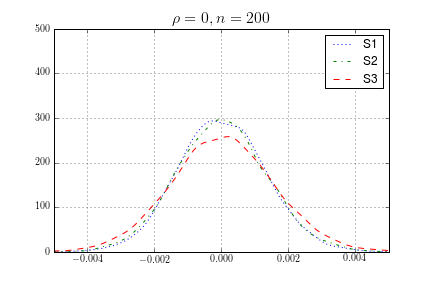
\includegraphics[width=8cm]{density_200_0} & 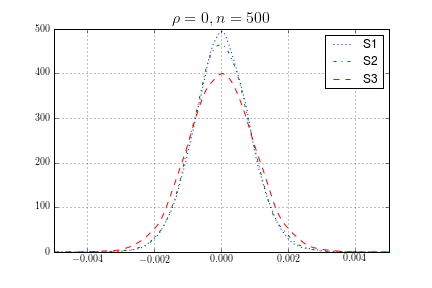
\includegraphics[width=8cm]{density_500_0} \\
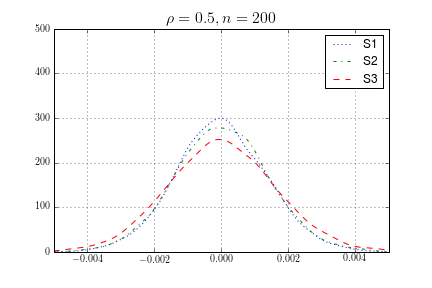
\includegraphics[width=8cm]{density_200_05} & 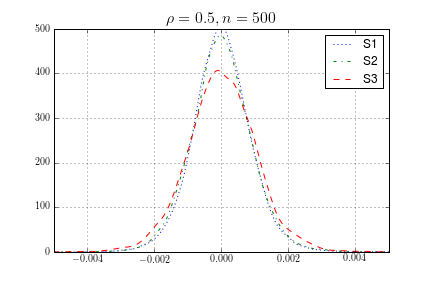
\includegraphics[width=8cm]{density_500_05} \\
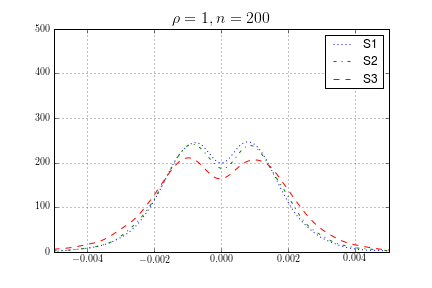
\includegraphics[width=8cm]{density_200_1} & 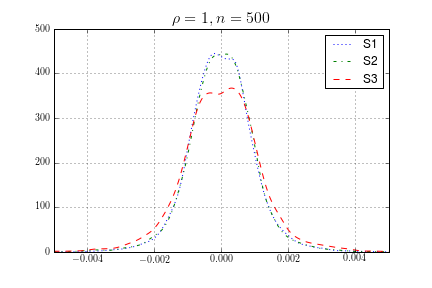
\includegraphics[width=8cm]{density_500_1} \\
\end{tabular}
}
\end{table}

\begin{table}[!ht]
\selectfont \caption{Density estimate of $\hat{\theta}_n$ (scaled by $n^{1/4}$).}
\label{GseqTable} \center{
\begin{tabular}{c c}
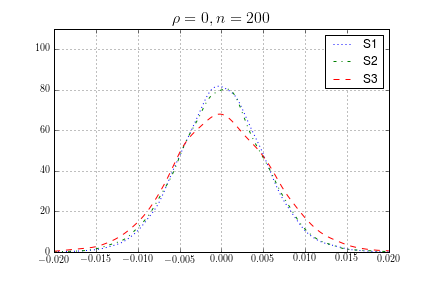
\includegraphics[width=8cm]{scaled_density_200_0} & 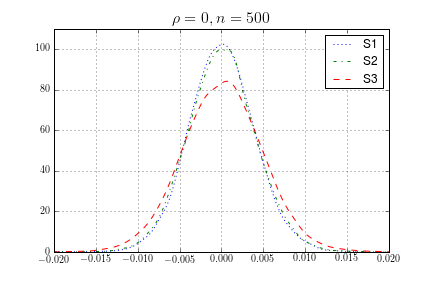
\includegraphics[width=8cm]{scaled_density_500_0} \\
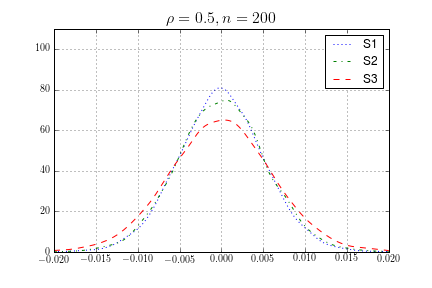
\includegraphics[width=8cm]{scaled_density_200_05} & 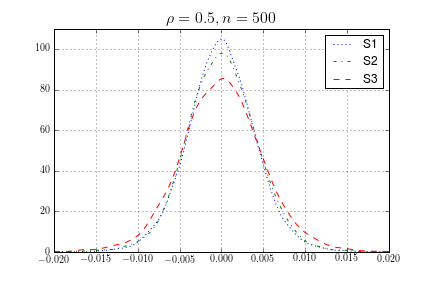
\includegraphics[width=8cm]{scaled_density_500_05} \\
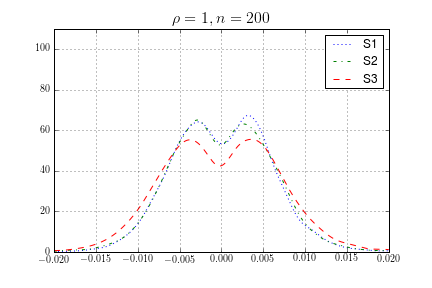
\includegraphics[width=8cm]{scaled_density_200_1} & 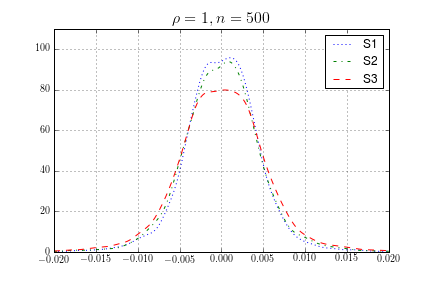
\includegraphics[width=8cm]{scaled_density_500_1} \\
\end{tabular}
}
\end{table}

\begin{table}[!ht]
\selectfont \caption{Density of $\hat{\theta}_n$ $t$-ratios.}
\label{GseqTable} \center{
\begin{tabular}{c c}
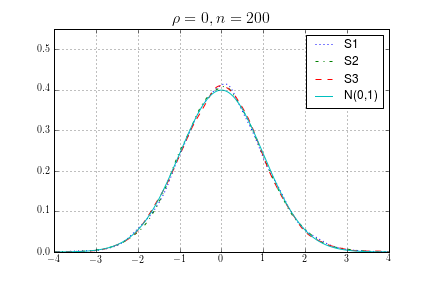
\includegraphics[width=8cm]{t_ratio_200_0} & 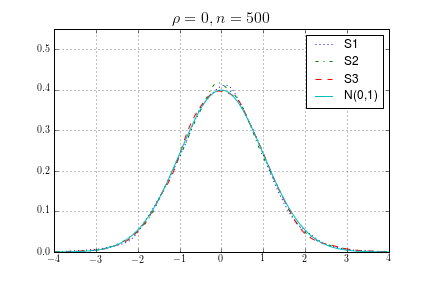
\includegraphics[width=8cm]{t_ratio_500_0} \\
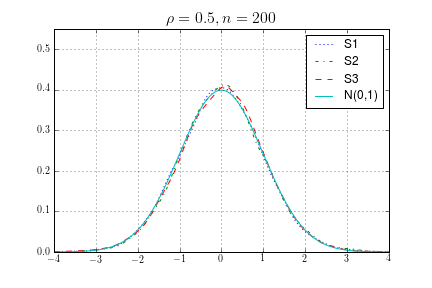
\includegraphics[width=8cm]{t_ratio_200_05} & 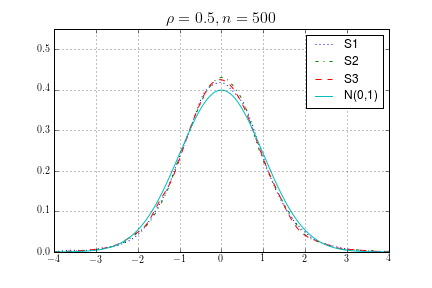
\includegraphics[width=8cm]{t_ratio_500_05} \\
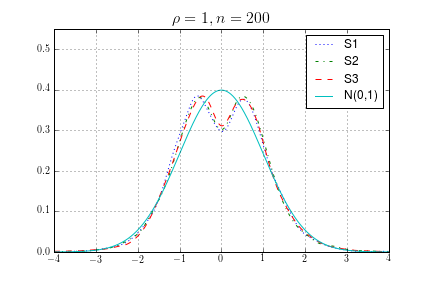
\includegraphics[width=8cm]{t_ratio_200_1} & 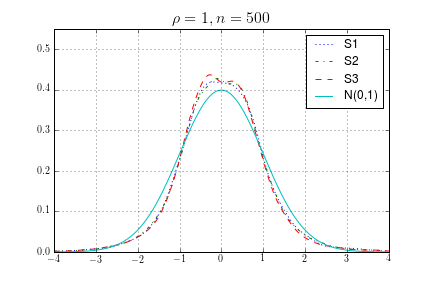
\includegraphics[width=8cm]{t_ratio_500_1} \\
\end{tabular}
}
\end{table}
%%%%%%%%%%%%%%%%%%%%%%%%%%%%%%%%%%%%%%
%                                    %
%                                    %
%            Conclusion              %
%                                    %
%                                    %
%%%%%%%%%%%%%%%%%%%%%%%%%%%%%%%%%%%%%%

\section{Conclusion}

In this paper, we establish an asymptotic theory for a nonlinear parametric cointegrating model. A general framework is developed for establishing the weak consistency of the NLS estimator $\hat{\theta}_n$. The framework can easily be applied to a wide class of nonstationary regressors, including the partial sum of linear process and Harris recurrent Markov chain. Limit distribution of $\hat{\theta}_n$ is also established, and thus significantly extend previous works. Furthermore, we introduce endogeneity to our model by allowing the error term serially dependent on itself, and cross-dependent on the regressor. We show that the limit distribution of $\hat{\theta}_n$ under the endogeneity situation is different from that with martingale error structure. This result is of interest in the applied econometric research area.


%%%%%%%%%%%%%%%%%%%%%%%%%%%%%%%%%%%%%%
%                                    %
%                                    %
%       Proofs of main results       %
%                                    %
%                                    %
%%%%%%%%%%%%%%%%%%%%%%%%%%%%%%%%%%%%%%

\section{Appendix A: Proofs of main results}

This section provides proofs of the main results. We start with some preliminaries, which list the limit theorems in common use in the proofs of main results.

\subsection{Preliminaries}

Denote $\mathcal N_{\de}(\pi_0) = \{ \theta: \| \theta - \pi_0\| < \de\}$, where $\pi_0 \in \Theta$ is fixed.
\begin{lem} \la{lemClose}
 Under (\ref {eqn:6:20}) and Assumption \ref{assump:6:Convex},   we have
\be \la{lemClose.eqn0}
\sup_{\theta \in \mathcal N_{\de}(\pi_0)} \kappa_n^{-2} \sum_{t = 1}^n \big(|f(x_t, \theta) - f(x_t, \pi_0)| + |f(x_t, \theta) - f(x_t, \pi_0)|^2\big)  &\to_P& 0
\ee
as $n\to\infty$ first and then $\de \to 0$. If in addition Assumption \ref{assump:6:Martingale}, then
\be \la{lemClose.eqn1}
\sup_{\theta \in \mathcal N_{\de}(\pi_0)}  \kappa_n^{-2} \sum_{t = 1}^n |[f(x_t, \theta) - f(x_t, \pi_0)]|\, |u_t|  \to_P 0
\ee
as $n\to\infty$ first and then $\de \to 0$.
\end{lem}

{\it Proof.} Simple and the details are omitted. $\Box$

\begin{lem} \la{lemC}
 Under Assumptions \ref{ad1} (i) and  \ref {ad2},   we have
\be \la{lemC.eqn1}
\frac {d_n}n\,\sup_{\theta \in \mathcal N_{\de}(\theta_0)}
\sum_{t = 1}^n \big|\dot f_i(x_t, \theta)\,\dot f_j(x_t, \theta) - \dot f_i(x_t, \theta_0)\,\dot f_j(x_t, \theta_0)\big|  &\to_P& 0, \\
\frac {d_n}n\,\sup_{\theta \in \mathcal N_{\de}(\theta_0)}\la{lemC.eqn2}
\sum_{t = 1}^n \big|\ddot f_{ij}(x_t, \theta)\,[ f(x_t, \theta) -  f(x_t, \theta_0)]\big|  &\to_P& 0.
\ee
as $n\to\infty$ first and then $\de \to 0$,  for any $1\le i, j\le m$. If in addition Assumption \ref{ad1} (ii)--(iii), then
\be\la{lemC.eqn3}
\frac {d_n}n\,\sup_{\theta \in \mathcal N_{\de}(\theta_0)}\big| \sum_{t = 1}^n\ddot f_{ij}(x_t, \theta)\,u_t \big| \to_P 0
\ee
as $n\to\infty$ first and then $\de \to 0$,  for any $1\le i, j\le m$.

The results are still true if Assumption \ref{ad1} (i) and \ref{ad2} are replaced by \ref{ad1}* (i) and \ref{ad2}* respectively, and $d_n / n$ is replaced by $a(n)^{-1}$.
\end{lem}

{\it Proof.} First note that, by Assumption \ref{ad2},
\begin{align}
\sup_{\theta \in \Theta} |f_i(x_t, \theta)| &\le \sup_{\theta \in \Theta} |\dot{f}_i(x_t, \theta)-\dot{f}_i(x_t, \theta_0)| + |\dot{f}_i(x_t, \theta_0)| \no\\
 &\le \sup_{\theta \in \Theta} h(\| \theta - \theta_0\|)T(x_t) + |\dot{f}_i(x_t, \theta_0)| \le C \no
\end{align}
It follows that
\bestar
&& \big|\dot f_i(x_t, \theta)\,\dot f_j(x_t, \theta) - \dot f_i(x_t, \theta_0)\,\dot f_j(x_t, \theta_0)\big| \no\\
&\le& \big|\dot f_i(x_t, \theta) \big |\big|\dot f_j(x_t, \theta)- \dot f_j(x_t, \theta_0)\big| + \big|\dot f_j(x_t, \theta_0) \big |\big|\dot f_i(x_t, \theta) - \dot f_i(x_t, \theta_0)\big| \no\\
&\le& C\big|\dot f_j(x_t, \theta)- \dot f_j(x_t, \theta_0)\big| +C_1\big|\dot f_i(x_t, \theta) - \dot f_i(x_t, \theta_0)\big|
\eestar
Therefore, (\ref{eqn:6:lemC.eqn1}) follows immediately from Lemma \ref{lemClose}. (\ref{eqn:6:lemC.eqn2}) is similar to (\ref{eqn:6:lemC.eqn1}) and thus we omit the details.

For (\ref{eqn:6:lemC.eqn3}), note that, for any $\theta \in \mathcal N_{\de}(\theta_0)$, $1 \le i, j \le m$,
\bestar
\Big |  \sum_{t = 1}^n \ddot{f}_{ij}(x_t, \theta) u_t \Big | &\le& \Big |   \sum_{t = 1}^n [\ddot{f}_{ij}(x_t, \theta) - \ddot{f}_{ij}(x_t, \theta_0)]\, u_t \Big |  + \Big |   \sum_{t = 1}^n  \ddot{f}_{ij}(x_t, \theta_0) u_t\Big | \no
\eestar
Then by (\ref{eqn:6:lemClose.eqn1}) in Lemma \ref{lemClose} (with $\pi_0  = \theta_0$) and Lemma \ref{lemJoint} below, we obtain the required (\ref{eqn:6:lemC.eqn3}).

 Finally, it can be easily seen that if Assumption \ref{ad1} (i) and \ref{ad2} are replaced by \ref{ad1}* (i) and \ref{ad2}* and $d_n / n$ replaced by $a(n)^{-1}$, the above arguments will hold true, due to Lemma \ref{lemMarkov} instead of Lemma \ref{lemJoint}.
 $\Box$

\begin{lem} \la{lemJoint} Suppose Assumption \ref{ad1} holds. Then, for any $g(x)$ and $g_1(x)$ satisfying
 $\int_{-\infty}^{\infty} (|g(x)|+|g(x)|^{4+\gamma})dx < \infty$ for some $\gamma > 0$,
  $\int_{-\infty}^{\infty} (|g_1(x)|+|g_1(x)|^{2})dx < \infty$,
 $\int_{-\infty}^{\infty} g(x) dx  \ne 0$ and $\int_{-\infty}^{\infty} g_1(x) dx  \ne 0$, we have
\be \la{lemJoint.eqn1}
\Big \{ \big(\frac {d_n}n\big)^{1/2}\sum_{t=1}^n g(x_t) u_t ,\, \frac {d_n}n\sum_{t=1}^n g_1(x_t) \Big \} &\rightarrow_D& \Big \{\tau_1 \, N \, L^{1/2}_{G}(1,0), \tau_2\, L_{G}(1,0) \Big \},
\ee
 where $\tau_1^2 = \int_{-\infty}^{\infty} g^2(s) ds$, $\tau_2= \int_{-\infty}^{\infty} g_1(s) ds$ and $N$ is a standard normal variate independent of $G(t)$.
\end{lem}

{\it Proof.}   Theorem 2.2 of \cite{wang2011} provides  (\ref {eqn:6:lemJoint.eqn1}) with $g_1(x)=g^2(x)$. It is not difficult to see that (\ref {eqn:6:lemJoint.eqn1}) still holds for general $g_1(x)$. We omit the details.  $\Box$

\begin{lem} \la{lemLagJoint} Under Assumption \ref {4.1}, for any bounded $g_i(x), i=1,2,$
satisfying $\int_{-\infty}^{\infty} |g_i(x)|dx < \infty$ and $\int_{-\infty}^{\infty} g_i(x) dx  \ne 0$, then
\be \la{lemLagJoint.eqn1}
 \sum_{t = 1}^n g_1(x_t) |u_t| = O_P(n / d_n)
\ee
and
\be \la{lemLagJoint.eqn2}
&\Big \{ (n/d_n)^{-1/2}\sum_{t=1}^n g_1(x_t) u_t ,\, (n/d_n)^{-1}\sum_{t=1}^n g_2(x_t) \Big \} \no\\
&\quad \rightarrow_D \Big \{\tau_3 \, N \, L^{1/2}_{G}(1,0), \tau_4 L_{G}(1,0) \Big \}
\ee
 where $\tau_3^2 = (2\pi)^{-1}\int_{-\infty}^{\infty}\hat{g_1}(\mu)^2 [ Eu_0^2 + 2 \sum_{r = 1}^{\infty}E(u_0u_r e^{-i\mu x_r})]\,d\mu$, $\hat{g_1}(\mu)=\int_{-\infty}^{\infty}e^{i\mu x}g_1(x) dx$ and $\tau_4 = \int_{-\infty}^{\infty} g_2(s) ds$.
\end{lem}

{\it Proof.} See Theorem 3 and 5 of \cite{jaganathan2008}. $\Box$

\begin{lem} \la{lemMarkov} Under Assumption \ref {ad1}* (i), for any $g$ such that $\int_{-\infty}^{\infty} |g(x)| \pi(dx) < \infty$ and $\int_{-\infty}^{\infty} g(x) \pi(dx) \ne 0$, we have
\be
\sum_{t = 1}^n g(x_t) &=& O_P[a(n)], \quad
\big [\sum_{t = 1}^n g(x_t)\big ]^{-1} = O_P[a(n)^{-1}] \la{eqn:6:ty}
\ee
If in addition Assumption \ref{ad1}* (ii)--(iv), for any bounded $g_i(x), i=1,2,$
satisfying $\int_{-\infty}^{\infty} |g_i(x)| \pi(dx) < \infty$ and $\int_{-\infty}^{\infty} g_i(x) \pi(dx)  \ne 0$, we have
\be \la{lemMarkov.eqn2}
\Big \{ a(n)^{-1/2}\sum_{t=1}^n g_1(x_t) u_t ,\, a(n)^{-1}\sum_{t=1}^n g_2(x_t) \Big \}  \rightarrow_D   \Big \{\tau_5 \, N \, \Pi^{1/2}_{\beta}, \tau_6\,\Pi_\beta \Big \}
\ee
 where $\tau_5^2 = \int_{-\infty}^{\infty} g_1^2(s) \pi(ds)$, $\tau_6= \int_{-\infty}^{\infty} g_2(s) \pi(ds)$ and $N$ is a standard normal variate independent of $\Pi$.
\end{lem}

{\it Proof.} The proof of (\ref {eqn:6:ty}) sees Theorem 2.1 of \cite{chen1999}. To prove (\ref{eqn:6:lemMarkov.eqn2}), we first impose an additional assumption that $g_2(x) = g_1^2(x)$. Denote
\be
\Delta^2_n = a(n)^{-1}\sum_{t = 1}^n g_1^2(x_t), \quad Z_{nt} = a(n)^{-1/2}g_1(x_t) \Delta_n^{-1}, \quad W_n = \sum_{t = 1}^n Z_{nt} u_k
\ee
Recalling that $E(u_t|\F_{nt}) = 0$, it is readily seen that given $\{x_1, ..., x_n\}$, $\{Z_{nt} u_t, \F_{nt}\}_{t = 1}^n$ forms a martingale difference sequence. The result (\ref{eqn:6:lemMarkov.eqn2}) will follow if we prove, 
\be \la{prfMarkov.eqn1}
\sup_{x} \big | P\big ( W_n \le x \, | \, x_1, ..., x_n \big ) - \Phi(x) \big | \to_P 0
\ee
%\begin{align}
%\sum_{t = 1}^n |Z_{nt}|^q &\to_P 0, \\
%\sum_{t = 1}^{\tau_n(t)} Z_{nt}^2 \,E(u_t^2 | \F_{nt}) &\to_P t,
%\end{align}
%for all $t \in [0, 1]$.

\noindent Indeed, by noting that $\Delta_n^2$ is measurable with respect to $\si(x_1,...x_n)$, we have, for any $\al, \gamma \in R$,
\begin{align}
&\big |E \big [ e^{i  \al  W_n + i \beta \Delta_n^2} \big ] - e^{-\frac{1}{2} \al^2 } \, E\big [e^{i \beta \tau_5 \Pi_\gamma} \big ] \big| \no\\
&\le E \Big |E \big ( e^{i \al W_n } |\, x_1, ..., x_n \big ) - e^{-\frac{1}{2}\al^2 } \,  \Big| +e^{-\frac{1}{2}\al^2}\Big| Ee^{i \gamma \Delta_n^2} - Ee^{i \gamma \tau_5 \Pi_\beta} \Big | \to 0 \no
\end{align}
by dominated convergence theorem, due to (\ref{eqn:6:prfMarkov.eqn1}) and $\Delta_n^2 \to_D \tau_5 \Pi_\beta$ (see, e.g., Theorem 2.3 of \cite{chen1999}). This implies that
\bestar
\{ W_n, \Delta_n^2 \} \to_D \{N, \tau_5\Pi_\beta\}
\eestar
where $N$ is a standard normal random variable independent of $\Pi_\beta$. Hence, by continuous mapping theorem, we have 
\bestar
\Big \{ a(n)^{-1/2}\sum_{t=1}^n g_1(x_t) u_t ,\, a(n)^{-1}\sum_{t=1}^n g_1^2(x_t) \Big \} = \Big \{ \Delta_n W_n, \Delta_n^2\Big \}\to_D \{\tau_5^{1/2} N\Pi_\beta^{1/2}, \tau_5\Pi_\beta\}
\eestar
which implies the required (\ref{eqn:6:lemMarkov.eqn2}).

We now prove (\ref{eqn:6:prfMarkov.eqn1}). By Theorem 3.9 ((3.75) there) in \cite{hallheyde1980} with $\de = q/2 - 1$ that
\bestar
\sup_{x} \big | P\big ( W_n \le x \, | \, x_1, ..., x_n \big ) - \Phi(x) \big | \le A(\de) \mathcal L_n^{1 / (1 + q)}  \quad a.s.
\eestar
where $A(\de)$ is a constant depending only on $\de$ and $q > 2$, and (set $\F^*_n = \si(x_1, ..., x_n)$)
\bestar
\mathcal L_n = \Delta_n^{-q} \sum_{k = 1}^n |Z_{nk}|^q E(|u_k|^q | \F^*_{n}) + E \Big [ \big | \Delta_n^{-2} \sum_{k = 1}^n Z_{nk}^2 [E(u_k^2 | \F_{nk}) - 1] \big|^{q/2} \Big | \, \F^*_{n} \Big].
\eestar
Recall from Assumption \ref{ad2} (iv) and the fact that $\Delta_n^2 = \sum_{k = 1}^n Z^2_{nk}$, we have,
\bestar
E \Big [ \big | \Delta_n^{-2} \sum_{k = 1}^n Z_{nk}^2 [E(u_k^2 | \F_{nk}) - 1] \big|^{q/2} \Big | \, \F^*_{n} \Big] \to_P 0
\eestar
by dominated convergence theorem. Hence,  routine calculations show that
\bestar
\mathcal L_n \le C\,\Delta_n^{-(q-2)} \,a(n)^{-(q-2)/2} + o_P(1) = o_P(1)
\eestar
because $\Delta_n^{-2}=O_P(1)$ by (\ref{eqn:6:ty}) and $q > 2$. This proves (\ref{eqn:6:prfMarkov.eqn1}), which implies that (\ref{eqn:6:lemMarkov.eqn2}) holds true with $g_2(x) = g_1^2(x)$. Finally, note that, for any $a$, $b \in R$,
\bestar
a(n)^{-1} \sum_{t = 1}^n \big \{ a g_1^2(x_t) + bg_2(x_t)\big  \}  \to_D  \int_{-\infty}^{\infty} \big [a g_1^2(s) + bg_2(s) \big ] \pi(ds)\, \Pi_\beta
\eestar
due to Theorem 2.3 of \cite{chen1999}, which implies that
\bestar
\Big \{ a(n)^{-1}\sum_{t=1}^n g_1^2(x_t) ,\, a(n)^{-1}\sum_{t=1}^n g_2(x_t) \Big \}\to_D  \Big \{\int_{-\infty}^{\infty} g_1^2(s) \pi(ds)\, \Pi_\beta, \int_{-\infty}^{\infty} g_2(s) \pi(ds)\, \Pi_\beta, \Big \}
\eestar
Hence, by continuous mapping theorem,
\bestar
\frac{ \sum_{t=1}^n g_1^2(x_t) }{\sum_{t=1}^n g_2(x_t)} \to_P \int_{-\infty}^{\infty} g_1^2(s)\,  \pi(ds) \Big /  \int_{-\infty}^{\infty} g_2(s) \, \pi(ds) 
\eestar
This shows that (\ref{eqn:6:lemMarkov.eqn2}) is still true with general $g_2(x)$. $\Box$

\begin{lem} \la{lemWu} Let $D_n(\theta, \theta_0) =  Q_n(\theta) - Q_n(\theta_0)$.
 Suppose that, for any $\de > 0$,
\be \la{lemWu.eqn1}
\liminf_{n \to \infty} \inf_{|\theta - \theta_0| \ge \delta} D_n(\theta, \theta_0) > 0 \quad in \quad  probability,
\ee
 then $\hat{\theta}_n \rightarrow_P \theta_0$.
\end{lem}

{\it Proof.} See Lemma 1 of \cite{wu1981}. $\Box$



\subsection{Proof of Theorems}

{\bf Proof of Theorem \ref {thmConsistency}.} Let $\mathcal N$ be any open subset of $\Theta$ containing $\theta_0$. Since $\hat{\theta}_n$ is the minimizer of $Q_n(\theta)$ in $\Theta$, therefore, by Lemma \ref{lemWu}, proving consistency is equivalent to showing that, for any $0<\eta<1$ and $\theta \ne \theta_0$, where $\theta, \theta_0\in \Theta$, there exist
 $n_0 > 0$ and $M_1>0$ such that
\be \la{prfConsistency.eqn1}
P \Big ( \inf_{\theta \in \Theta \cap \mathcal N^c}\, D_n(\theta, \theta_0) \ge  \kappa^2_n /M_1 \Big ) \ge 1 - \eta
\ee
for all $n > n_0$.

Denote $\mathcal N_{\de}(\pi_0) = \{ \theta: \| \theta - \pi_0\| < \de\}$. Note that $\Theta \cap \mathcal N^c$ is compact, by the finite covering property of compact set, (\ref{eqn:6:prfConsistency.eqn1}) will follow if we prove that, for any fixed $\pi_0 \in \Theta \cap \mathcal N^c$,
\be \la{prfConsistency.eqn2}
\sup_{\theta \in \mathcal N_{\de}(\pi_0)} \kappa_n^{-2} \Big | D_n(\theta, \theta_0) - D_n(\pi_0, \theta_0) \Big | \to_P 0
\ee
as $n\to\infty$ first and then $\de \to 0$, and for $\forall \ep>0$, there exists $M_1 > 0$ and $n > n_0$ such that for all $n > n_0$,
\be \la{prfConsistency.eqn3}
P\Big ( D_n(\pi_0, \theta_0) \ge \kappa^2_n/M_1 \Big ) \ge 1 -2 \eta.
\ee
The result  (\ref{eqn:6:prfConsistency.eqn2}) is simple. Indeed, by Lemma \ref{lemClose}, it follows that, for each fixed $\pi_0 \in \Theta \cap \mathcal N^c$,
\begin{align}
&\sup_{\theta \in \mathcal N_{\de}(\pi_0)}\kappa_n^{-2}\Big | D_n(\theta, \theta_0) - D_n(\pi_0, \theta_0) \Big | \no\\
&=\sup_{\theta \in \mathcal N_{\de}(\pi_0)} \kappa_n^{-2}\sum_{t=1}^n (f(x_t, \theta) - f(x_t, \pi_0))^2 \no\\
&\hskip 3.5cm - \sup_{\theta \in \mathcal N_{\de}(\pi_0)}\kappa_n^{-2} \sum_{t = 1}^n |f(x_t, \theta) - f(x_t, \pi_0)|| u_t|\no\\
&\to_P 0
\end{align}
as $n\to\infty$ first and then $\de \to 0$, which yields (\ref {eqn:6:prfConsistency.eqn2}).

To prove (\ref{eqn:6:prfConsistency.eqn3}), we  write
\bestar
D_n(\pi_0, \theta_0) =  \sum_{t = 1}^n (f(x_t, \pi_0) - f(x_t, \theta_0))^2 -  \sum_{t = 1}^n (f(x_t, \pi_0) - f(x_t, \theta_0)) u_t
\eestar
Similar arguments as in Lemma \ref{lemClose} yields that
\bestar
\sum_{t = 1}^n (f(x_t, \pi_0) - f(x_t, \theta_0)) u_t = o_P(\kappa^2_n)
\eestar
Hence, it follows from Assumption \ref{assump:6:LowerBound} that,
 for any $\eta>0$, there exists $n_0 > 0$ and $M_1 > 0$ such that for all $n > n_0$,
\begin{align}
P\Big ( D_n(\pi_0, \theta_0) \ge M_1^{-1} \Big ) &\ge P \Big ( \sum_{t = 1}^n ( f(x_t, \pi_0) - f(x_t, \theta_0))^2 \ge \kappa^2_n\, M_1^{-1}/2 \Big ) - \eta \no\\
&\ge1 -2 \eta \no
\end{align}
which implies (\ref{eqn:6:prfConsistency.eqn3}).

Finally for the error estimate $\hat{\si}_n^2$, note that by Assumption \ref{assump:6:Martingale} and strong law of large number, $Q(\theta_0) = n^{-1} \sum_{t = 1}^n u_t^2 \to_P \si^2$. Then it immediately follows from the consistency of $\hat{\theta}_n$ and (\ref{eqn:6:prfConsistency.eqn2}) that 
\bestar
|\hat{\si}_n^2 - \si^2| \le C \kappa_n^{-2} |Q_n(\hat{\theta}_n) - Q_n(\theta_0)| + o_P(1) = o_P(1).
\eestar
$\Box$


\medskip
{\bf Proof of Theorem \ref {thmLinearConsistency}.}
 It follows from Lemma \ref{lemJoint} that
\bestar
\frac{d_n}{n} \sum_{t = 1}^n (f(x_t, \theta) - f(x_t, \theta_0))^2  \rightarrow_D \Big ( \int_{-\infty}^{\infty} (f(s, \theta) - f(s, \theta_0))^2 ds \Big ) L_{G}(1,0)
\eestar
 where \be
 G(t) &=&\begin{cases}
 W_{\mu - 3/2}(t),  & \mbox{under C1,} \\
W(t), & \mbox{under C2.}
\end{cases} \la{eqn:6:im19}
\ee
The result (\ref{eqn:6:21}) follows from the well known fact that $P(L_G(1,0) > 0) = 1$ and $\int_{-\infty}^{\infty} (f(s, \theta) - f(s, \theta_0))^2 ds > 0$, for any $\theta \ne \theta_0$.

By noting $E[T(x_k)+T^2(x_k)]\le C\, d_k^{-1}$ due to Lemma 3.2 of \cite{wangphillips2009}, simple calculations show that
\bestar
\frac {d_n}n \sum_{k=1}^n E[T(x_k)+T^2(x_k)] \le C\,
\eestar
which implies (\ref {eqn:6:20}). $\Box$


\medskip
{\bf Proof of Theorem \ref {thmMarkovConsistency}.} The results (\ref {eqn:6:20}) and (\ref {eqn:6:21}) follow from Lemma \ref{lemMarkov} with $g(x)=T(x)+T^2(x)$ and $g(x)=(f(x, \theta)-f(x, \theta_0))^2$, respectively. $\Box$


\medskip
{\bf Proof of Theorem \ref {thmHomoConsistent1}.} The proof  is essentially the same as that given in Theorems 4.2 and 4.3 of PP. We only provide a outline for $f(x, \theta)$
satisfying the {\bf Case 2}, which is related to the verification of the conditions in Lemma \ref{lemWu}.

 Let $\Theta_0 = \{ \| \theta - \theta_0 \| \ge \de \}$ where  $\de>0$ is a constant.
By virtue of Lemma \ref{lemWu},   it suffices to prove that, for any $\eta, M_0 >0$, there exist a $n_0 >0$ such that, for all $n > n_0$,
\be \la{prfHomoConsistent2.eqn1}
P \Big (n^{-1} \inf_{\theta \in \Theta_0} D_n(\theta, \theta_0) > M_0 \Big ) > 1-  \eta.
\ee
To prove (\ref{eqn:6:prfHomoConsistent2.eqn1}),  first note that  $\sum_{t=1}^nu_t^2/n\le M_0$ in probability, for some $M_0>0$, due to the Assumption 2.2 (i). This, together with Cauchy-Schwarz Inequality, yields that
\begin{align}
&n^{-1}D_n(\theta, \theta_0) \no\\
& \quad = \frac{1}{n} \sum_{t = 1}^n (f(x_t, \theta) - f(x_t, \theta_0))^2 - \frac{2}{n} \sum_{t = 1}^n (f(x_t, \theta) - f(x_t, \theta_0))u_t  \no\\
&\quad \ge \frac{1}{n} \sum_{t = 1}^n (f(x_t, \theta) - f(x_t, \theta_0))^2 - \frac{2}{n}\Big ( \sum_{t = 1}^n (f(x_t, \theta) - f(x_t, \theta_0))^2 \Big )^{1/2} \Big (\sum_{t = 1}^n u^2_t \Big )^{1/2}  \no\\
&\quad \ge M_n(\theta, \theta_0)\Big [1  - \frac{2\sqrt{M_0 + o_P(1) }}{M_n(\theta, \theta_0 )^{1/2} } \Big ] ,
\end{align}
where $M_n(\theta, \theta_0)=
 \frac{1}{n} \sum_{t = 1}^n (f(x_t, \theta) - f(x_t, \theta_0))^2$. Hence, for any equivalent process $x_{k}^*$ of $x_k$ (i.e., $x_{k}^*=_d x_{k}, 1\le
k\le n, n\ge 1$, where $=_d$ denotes equivalence in distribution), we have
\be
P \Big (n^{-1} \inf_{\theta \in \Theta_0} D_n(\theta, \theta_0) > M_0 \Big ) \ge
P \Big (\inf_{\theta \in \Theta_0}M_n^*(\theta, \theta_0)\Big [1  - \frac{2\sqrt{M_0 + o_P(1) }}{M_n^*(\theta, \theta_0 )^{1/2} } \Big ] >M_0 \Big ), \la{eqn:6:14}
\ee
where $M_n^*(\theta, \theta_0)= \frac{1}{n} \sum_{t = 1}^n (f(x_t^*, \theta) - f(x_t^*, \theta_0))^2$.

Recalling $x_{[nt]}/d_n\Rightarrow G(t)$ on $D[0,1]$ and
 $G(t)$ is a continuous
Gaussian process, by the so-called
Skorohod-Dudley-Wichura representation theorem (e.g., \cite[][p. 49, Remark 2]{shorackwellner1986}, we can choose an equivalent process $x_{k}^*$ of $x_k$  so that
\be
	\sup_{0\le t\le 1}|x_{[nt]}^*/d_n-G(t)| &=&o_P(1). \la{eqn:6:a17}
\ee
For this equivalent process $x_t^*$, it follows from the structure of $f(x,\theta)$  that
\be \la{190}
m(d_n, \theta)^2 &:=& \frac{1}{n v(d_n, \theta)^2} \sum_{t = 1}^n f(x_t^*, \theta)^2\no\\
&=&\frac{1}{n } \sum_{t = 1}^n h(x_t^*/d_n, \theta)^2 +o_P(1) \no\\
&=&  \int_0^1 h(x_{[ns]}^*/d_n, \theta)^2ds+o_P(1) \no\\
&\to_P& \int_{0}^1 h(G(s), \theta)^2 ds =: m(\theta)^2,
\ee
uniformly in $\theta\in\Theta$. Due to (\ref {eqn:6:190}), the same arguments as in the proof of Theorem 4.3 in PP yields that
\bestar
\inf_{\theta \in \Theta_0}M_n^*(\theta, \theta_0) \to \infty, \quad \mbox{in probability,}
\eestar
which, together with (\ref {eqn:6:14}), implies (\ref {eqn:6:prfHomoConsistent2.eqn1}).
$\Box$




\medskip
{\bf Proof of Theorem \ref {thmIntegrablelimit}.} According to the introductory remark of Section 3, it suffices to verify the conditions (\ref{eqn:6:rmk1.1})--(\ref{eqn:6:rmk1.5}) with
\bestar
\kappa^2_n &=& n / d_n, \quad c_{i,j} = \int_{-\infty}^{\infty} \dot{f}_i(s, \theta_0) \dot{f}_j(s, \theta_0) ds / \int_{-\infty}^{\infty} f(s, \theta_0) ds, \no\\
Y &=& \Sigma^{1/2} \, \mbox{{\bf N}}L_G^{1/2}(1,0), \quad
Z = \int_{-\infty}^{\infty} f(s, \theta_0) ds\, L_G(1,0),
\eestar
under Assumptions \ref {ad1} and \ref {ad2}.

 Recalling $\hat\theta_n\to_P\theta_0$ due to Theorems 2.1 and 2.2,  $\hat{\theta}_n$
 falls in $\mathcal N_{\de}(\theta_0) = \{ \theta: \| \theta - \theta_0\| < \de\}$ in probability. This, together with Lemma \ref {lemC}, yields  (\ref{eqn:6:rmk1.1})--(\ref{eqn:6:rmk1.3}).

It follows from Lemma \ref{lemJoint} with $g(x)=\al'\dot{f}(x, \theta_0)$ and $g_1(x)=f(x, \theta_0)$ that
\be\la{prfIntegrablelimit.eqn5}
&& \Big \{ \Big (\frac{d_n}{n}\Big)^{1/2}\,\sum_{t=1}^n \al'\, \dot{f}(x_t, \theta_0) u_t ,\,\frac{d_n}{n}\sum_{t=1}^n f(x_t, \theta_0) \Big \} \no\\
&&\qquad \qquad \rightarrow_D  \Big \{\tau\,N\, L_G^{1/2}(1, 0), Z\Big \} =_D \Big \{ \al' \,Y, Z \Big \}
\ee
where $\tau^2 = \int_{-\infty}^{\infty} [\al'\dot{f}(s, \theta_0)]^2 ds $, $N$ is a standard normal random variable independent of $G(t)$ and we have used the fact that
\bestar
\tau\, N &=& \Big(\int_{-\infty}^{\infty} [\al'\dot{f}(s, \theta_0)]^2 ds\Big)^{1/2}\,  N \no\\
&=_D& \al' \Big(\int_{-\infty}^{\infty} \dot{f}(s, \theta_0)\dot{f}(s, \theta_0)' ds\Big)^{1/2}\, \mbox{{\bf N}} =\al'\, \Sigma^{1/2}\,\mbox{{\bf N}}.
\eestar
 This proves (\ref {eqn:6:rmk1.4}).

 Finally, it follows from Lemma \ref{lemJoint} with
  $g_1(x)=\beta_1\dot{f}_i(x, \theta_0) \dot{f}_j(x, \theta_0)+\beta_2f(x, \theta_0)$ that
 \bestar
\frac{d_n}{n}\sum_{t=1}^n
\big[\beta_1\dot{f}_i(x_t, \theta_0) \dot{f}_j(x_t, \theta_0)+\beta_2f(x_t, \theta_0)\big]\to_D \tau_0\, L_G(1,0),
\eestar
where $\tau_0= \int_{-\infty}^{\infty}\,\big[\beta_1\dot{f}_i(x, \theta_0) \dot{f}_j(x, \theta_0)+\beta_2f(x, \theta_0)\big] dx$. This yields  (\ref {eqn:6:rmk1.5}), that is,
\bestar
\Big \{  \frac{d_n}{n}\sum_{t=1}^n  \dot{f}_i(x_t, \theta_0)\dot{ f}_j(x_t, \theta_0),\,  \frac{d_n}{n}\sum_{t=1}^n f(x_t, \theta_0)\Big \}  \rightarrow_D \Big \{ c_{i,j}\,Z, Z\Big \}.
\eestar
$\Box$

{\bf Proof of Theorem \ref {thmIntegrablelimit1}. }
 As in Theorem \ref{thmIntegrablelimit}, we need to verify the conditions (\ref{eqn:6:rmk1.1})--(\ref{eqn:6:rmk1.5}), but with
\bestar
\kappa^2_n &=& a(n), \quad c_{i,j} = \int_{-\infty}^{\infty} \dot{f}_i(s, \theta_0) \dot{f}_j(s, \theta_0) \pi(ds) / \int_{-\infty}^{\infty} f(s, \theta_0) \pi(ds), \no\\
Y &=& \Sigma_\pi^{1/2} \, \mbox{{\bf N}}\Pi_\beta, \quad
Z = \int_{-\infty}^{\infty} f(s, \theta_0) \pi(ds)\, \Pi_\beta,
\eestar
under Assumptions \ref {ad1}* and \ref {ad2}*. The details are similar to that of Theorem \ref{thmIntegrablelimit}, with Lemma \ref{lemJoint} replaced by Lemma \ref{lemMarkov}, and hence are omitted. $\Box$

\medskip
{\bf Proof of Theorem \ref {11}.} We first establish the consistency result. The proof goes along the same line as in Theorem \ref{thmConsistency}. It suffices to show that for any fixed $\pi_0 \in \Theta \cap \mathcal N^c$, 
\be \la{prf11.eqn1}
\sup_{\theta \in \mathcal N_{\de}(\pi_0)} \frac{d_n}{n} \sum_{t = 1}^n |[f(x_t, \theta) - f(x_t, \pi_0)]u_t|  \to_P 0
\ee
as $\de\to 0$ uniformly for all large $n$, and
\be\la{prf11.eqn2}
\sum_{t = 1}^n (f(x_t, \pi_0) - f(x_t, \theta_0)) u_t = o_P(n/d_n).
\ee

For (\ref{eqn:6:prf11.eqn1}). By (\ref{eqn:6:lemLagJoint.eqn1}) in Lemma \ref{lemLagJoint} with $g_1(x) = |T(x)|$, we have,
\begin{align}
\sup_{\theta \in \mathcal N_{\de}(\pi_0)}\frac{d_n}{n} \sum_{t = 1}^n |[f(x_t, \theta) - f(x_t, \pi_0)]u_t| &\le \sup_{\theta \in \mathcal N_{\de}(\pi_0)} h(\|\theta- \pi_0\|) \,  \frac{d_n}{n} \sum_{t = 1}^n|T(x_t)|| u_t| \no\\
&\le C\, \sup_{\theta \in \mathcal N_{\de}(\pi_0)}h(\|\theta- \pi_0\|)\, O_P(1) \to_P 0 \no
\end{align}
as $\de \to 0$.

Also, by (\ref{eqn:6:lemLagJoint.eqn2}) in Lemma \ref{lemLagJoint} with $g_1(x) = f(x, \pi_0) - f(x, \theta_0)$, we have that
\bestar
\sum_{t = 1}^n (f(x_t, \pi_0) - f(x_t, \theta_0)) u_t = O_P[(n/d_n)^{1/2}]
\eestar
which implies the required (\ref{eqn:6:prf11.eqn2}) immediately.

We next give the limit distribution. As in Theorem \ref{thmIntegrablelimit}, we need to verify the conditions (\ref{eqn:6:rmk1.1})--(\ref{eqn:6:rmk1.5}), but with
\bestar
\kappa^2_n &=& n / d_n, \quad c_{i,j} = \int_{-\infty}^{\infty} \dot{f}_i(s, \theta_0) \dot{f}_j(s, \theta_0) ds / \int_{-\infty}^{\infty} f(s, \theta_0) ds, \no\\
Y &=& \Lambda^{1/2} \, \mbox{{\bf N}}L_G^{1/2}(1,0), \quad
Z = \int_{-\infty}^{\infty} f(s, \theta_0) ds\, L_G(1,0),
\eestar
under Assumptions \ref {4.1}.

The proof for (\ref{eqn:6:rmk1.1}), (\ref{eqn:6:rmk1.2}) and (\ref{eqn:6:rmk1.5}) are exactly same as that of Theorem \ref{thmIntegrablelimit}, and using similar arguments, (\ref{eqn:6:rmk1.4}) will follow from Lemma \ref{lemJoint}.

For (\ref{eqn:6:rmk1.3}). Because $\hat{\theta}_n \to_P \theta_0$, by (\ref{eqn:6:prf11.eqn1}) with $\pi_0 = \theta_0$, and (\ref{eqn:6:prf11.eqn2}), we have, for any $1 \le i,j \le m$,
\bestar
\Big |\frac{d_n}{n}  \sum_{t = 1}^n \ddot{f}_{ij}(x_t, \theta_n) u_t \Big | &\le& \Big | \frac{d_n}{n}  \sum_{t = 1}^n [\ddot{f}_{ij}(x_t, \theta_n) - \ddot{f}_{ij}(x_t, \theta_0)]\, u_t \Big |  + \Big | \frac{d_n}{n}  \sum_{t = 1}^n  \ddot{f}_{ij}(x_t, \theta_0) u_t\Big | \no\\
&=& o_P(1)
\eestar
which yields the required (\ref{eqn:6:rmk1.3}). $\Box$

\section{Appendix B: Definition of regular function} \la{app.regularDef}
$H$ is called a regular function if there exists for each $\epsilon > 0$ continuous functions $\underline{H}_\epsilon$, $\overline{H}_\epsilon$, and a constant $\delta_\epsilon > 0$ such that $\underline{H}_\epsilon(x) \le H(y) \le \overline{H}_\epsilon(x)$ for all $|x - y| < \delta_\epsilon$ on $K$, a compact set of $R$, and such that $\int_K (\overline{H}_\epsilon - \underline{H}_\epsilon)(x)dx \rightarrow 0$ as $\epsilon \rightarrow 0$.


%%% Local Variables: 
%%% mode: latex
%%% TeX-master: "../thesis"
%%% End: 
